\thispagestyle{fancy}

\section{A grafikus interfész}
A szoftver elindulásakor a játékos egy eltéveszthetetlenül egyszerű menüben fogja találni magát, ahol
választhat hogy hány játékos vegyen részt a játékban. Az egész játék, úgy ahogyan a menü is korunk csempe életérzését fogja tükrözni

\begin{figure}[h]
	\begin{center}
		
\includegraphics[width=5cm]{chapters/chapter11/StapelMenu.png}
		\caption{menu}
		\label{fig:Grafikus}
	\end{center}
\end{figure}

Miután a felhasználó kiválasztotta a játékosok számát a játék elindul. Az egész játék egy panelekre osztott játéktérben fog zajlani, ahol a játékos az egér segítségével tudja majd mozgatni a robotot, illetve csapdákat letenni vele.

\begin{figure}[h]
	\begin{center}
		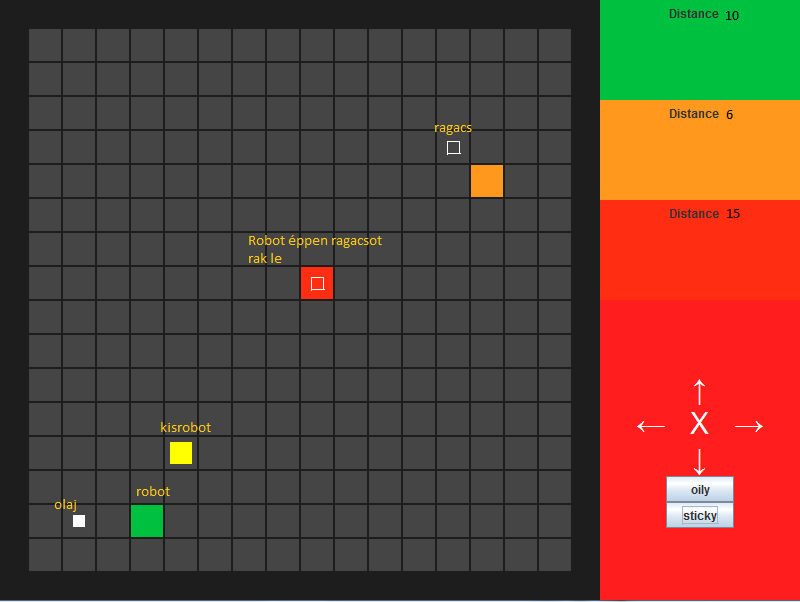
\includegraphics[width=17cm]{chapters/chapter11/StapelInGame.png}
		\caption{játék közben}
		\label{fig:Grafikus}
	\end{center}
\end{figure}


\section{A grafikus rendszer architektúrája}

\subsection{A felület működési elve}
	A Window osztály az egész felület containere, ez egy form egy jobb oldali, és egy bal oldali panelből áll. A bal oldali panel megjeleníthető a GameStartPanel osztály egy példányát, ebben az esetben
	a menü rajzolódik ki. A másik lehetőség hogy a GamePanel egy osztálya jelenik meg a bal oldalon,
	ami egy aktív játékteret ábrázol.
	A jobb oldali panel szintén container. Ez tartalmazza játék közben a felső részében eredménypanelt, illetve az alsó részében a vezérlő panelt.
	Indításnál a gamestartpanel a gombot action listenere is egyben. Ha a user klikkel, akkor gamecontroller elindítja a játékot, a megadott számú robottal, innentől a controller panel veszi át az input controller szerepét. 
	A controllerpanel listenerjei a gamecontroller függvényeit hívja meg. Léptetésnél a robotStep fogja léptetni a robot, a modellben elindítani a folyamatokat, és továbbadni a vezérlést a soron következő robotnak.
	
	Minden kirajzolandó játékbeli objektumhoz, tehát a Robot, Pálya, Ragacs és Olajfolt tartozik egy View Osztály is. Ez a View osztály végzi el az egyes elemek kirajzolását. A következő a folyamat: A modell változik a user input hatására, miután a model updatelődött a GamePanel újrarajzolódik, ami cserébe meghívja a View objektumot és a Panelek paintComponent metódusát, ami újrarajzolja a játékteret.
	 
	Az grafikus Architektura pull modellre épül, mert minden lépés után a grafikus interface lekéri a modellből a változásokat, és aktualizálja a grafikus interfacet.
	\clearpage
\subsection{A felület osztály-struktúrája}


\begin{figure}[h]
	\begin{center}
		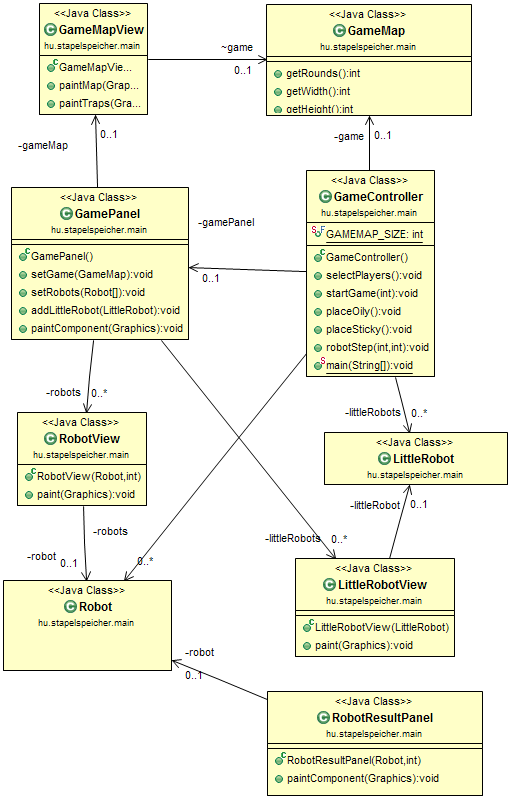
\includegraphics[width=11cm]{chapters/chapter11/StapelGrafUML1.png}
		\caption{Grafikus UML első fele}
		\label{fig:Grafikus}
	\end{center}
\end{figure}

\clearpage
\begin{figure}[h]
	\begin{center}
		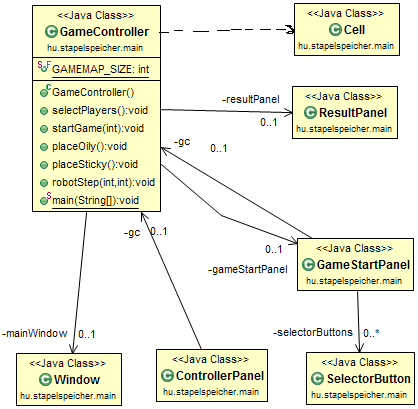
\includegraphics[width=14cm]{chapters/chapter11/StapelGrafUML2.png}
		\caption{Grafikus UML második fele}
		\label{fig:Grafikus}
	\end{center}
\end{figure}



